%\VignetteIndexEntry{erccdashboard examples}

\documentclass{article}
\usepackage{fullpage}
\usepackage{Sweave}
\begin{document}
\Sconcordance{concordance:erccdashboardVignette.tex:erccdashboardVignette.Rnw:%
1 4 1 1 0 8 1 1 7 33 1 1 2 4 0 1 2 19 1 1 2 13 0 1 2 %
23 1 1 2 1 0 8 1 1 2 1 0 1 1 3 0 1 2 29 1 1 7 130 0 1 %
2 5 1 1 2 21 0 1 2 4 1 1 2 5 0 1 2 7 1 1 2 5 0 1 2 7 %
1 1 2 5 0 1 2 8 1 1 2 5 0 1 2 15 1 1 7 142 0 1 2 1 1 %
1 2 5 0 1 2 7 1 1 2 6 0 1 1 7 0 1 2 1 1 1 2 5 0 1 2 %
14 1 1 2 5 0 1 2 7 1 1 2 5 0 1 2 20 1 1 7 75 0 1 2 1 %
1 1 2 5 0 1 2 5 1 1 2 5 0 1 2 8 1 1 2 5 0 1 2 9 1 1 2 %
5 0 1 2 17 1 1 2 38 0 1 2 58 1 1 2 36 0 1 2 1 1}



\DefineVerbatimEnvironment{Sinput}{Verbatim} {xleftmargin=1em}
\DefineVerbatimEnvironment{Soutput}{Verbatim}{xleftmargin=1em}
\DefineVerbatimEnvironment{Scode}{Verbatim}{xleftmargin=1em}
\fvset{listparameters={\setlength{\topsep}{0pt}}}
\renewenvironment{Schunk}{\vspace{\topsep}}{\vspace{\topsep}}
\title{{\tt erccdashboard} Package Vignette}
\author{Sarah A. Munro}
\maketitle

This vignette describes the use of the erccdashboard R package to analyze 
External RNA Control Consortium (ERCC) spike-in control ratio mixtures in gene
expression experiments. If you use this package for method validation of your
gene expression experiments please cite our manuscript that describes this R 
package.

In this vignette we demonstrate analysis of two types of gene expression experiments
from the SEQC project that used ERCC control ratio mixture spike-ins:
\begin{itemize}
  \item Rat toxicogenomics treatment and control samples for different drug
  treatments
  \item Human reference RNA samples from the MAQC I project, Universal Human 
  Reference RNA (UHRR) and Human Brain Reference RNA (HBRR)
\end{itemize}

A subset of the large data set produced in the SEQC study is provided here as 
examples. The three sets of example data are: 

\begin{enumerate}
  \item Rat toxicogenomics RNA-Seq gene expression count data
  \item UHRR/HBRR RNA-Seq gene expression count data
  \item UHRR/HBRR Microarray gene expression fluorescent intensity data
\end{enumerate}


\section{Rat Toxicogenomics Example: MET (methimazole treatment) and CTL 
(control) Experiment}
\subsection{Load data and define input parameters} 

Load the package gene expression data.
\begin{Schunk}
\begin{Sinput}
> data(SEQC.Example)
\end{Sinput}
\end{Schunk}

The R workspace should now contain 5 objects
Three of these objects are gene expression experiment expression measures:
\begin{itemize}
  \item Lab10.array.UHRR.HBRR - Fluorescent signal data from an Illumina 
        beadarray microarray experiment with UHRR and HBRR
  \item COH.RatTox.ILM.MET.CTL.countTable - RNA-Seq count data from a
        rat toxicogenomics experiment
  \item Lab5.ILM.UHRR.HBRR.countTable - RNA-Seq count data from Lab 5 in the SEQC
        interlaboratory study with UHRR and HBRR
\end{itemize}
The other two objects are vectors of total reads for the 2 sequencing experiments
\begin{itemize}
  \item COH.RatTox.ILM.MET.CTL.totalReads - total sequenced reads factors for 
        each column in the corresponding rat experiment count table
  \item Lab5.ILM.UHRR.HBRR.totalReads - total sequenced reads factors for 
        each column in the corresponding UHRR/HBRR count table
\end{itemize}

Take a look at the count table for the MET experiment.
\begin{Schunk}
\begin{Sinput}
> head(COH.RatTox.ILM.MET.CTL.countTable)
\end{Sinput}
\begin{Soutput}
         Feature MET_1 MET_2 MET_3 CTL_1 CTL_2 CTL_3
16499 ERCC-00002 16629 18798 26568 36600 45436 25163
16500 ERCC-00003  1347  1565  1983  3048  3447  2195
16501 ERCC-00004  4569  5570  6755  1240  1484   902
16502 ERCC-00009   811   869  1123   909  1073   537
16503 ERCC-00012     0     0     0     0     0     0
16504 ERCC-00013     3     1     2     1     5     1
\end{Soutput}
\end{Schunk}
The first column of the count table, Feature, contains unique names for all
the transcripts that were quantified in this experiment. The remaining columns 
represent replicates of the pair of samples, in this count table 
the control sample is labeled CTL and the treatment sample is labeled MET. An 
underscore is included to separate the sample names from the replicate numbers 
during analysis. This column name format Sample\textunderscore{}Rep is required 
for the columns of any input count table.

These RNA-Seq count tables also must be unnormalized count data, because the 
default differential expression testing of
RNA-Seq experiments in the erccdashboard is done with the QuasiSeq package, 
which requires the use of integer count data. During the erccdashboad analysis 
the input count data will be normalized using library size factors. These factors
can be provided by the user as the input argument repNormFactor, a 
vector of total reads. The example total reads vectors we provide here were
derived from the FASTQ files associated with each column in the count tables. 
Alternatively, if repNormFactor is undefined (or NULL) for an RNA-Seq analysis 
then a vector of total mapped reads (column sums of a count table) will be 
calculated and used for normalization. 

\subsection{Quick analysis: runDashboard}
To run the default analysis function runDashboard on the MET-CTL rat 
toxicogenomics RNA-Seq experiment, the following input arguments are required:

\begin{Schunk}
\begin{Sinput}
> datType = "count" # "count" for RNA-Seq data, "array" for microarray data
> isNorm = FALSE # flag to indicate if input expression measures are already normalized, default is FALSE
> exTable = COH.RatTox.ILM.MET.CTL.countTable # the expression measure table
> filenameRoot = "COH.ILM" # user defined filename prefix for results files
> sample1Name = "MET" # name for sample 1 in the experiment
> sample2Name = "CTL" # name for sample 2 in the experiment
> erccmix = "RatioPair" # name of ERCC mixture design, "RatioPair" is default
> erccdilution = 1/100 # dilution factor used for Ambion spike-in mixtures
> spikeVol = 1 # volume (in microliters) of diluted spike-in mixture added to 
>              #   total RNA mass
> totalRNAmass = 0.500 # mass (in micrograms) of total RNA 
> choseFDR = 0.1 # user defined false discovery rate (FDR), default is 0.05
\end{Sinput}
\end{Schunk}

The first input argument, datType, indicates whether that data is integer count data from an RNA-Seq experiment ("count") or data from a microarray experiment ("array"). The isNorm argument indicates if the input expression measures are already normalized, default is FALSE.
The exTable argument is the expression measure table.

For any experiment the sample spiked with ERCC Mix 1 is sample1Name and the 
sample spiked with ERCC Mix 2 is sample2Name. In this experiment 
sample1Name = MET and sample2Name = CTL. For a more robust experimental design 
the reverse spike-in design could be created using additional replicates of the
treatment and control samples. ERCC Mix 2 would be spiked into MET samples and 
ERCC Mix 1 would be spiked into CTL control replicates. 

The dilution factor of the pure Ambion ERCC mixes prior to spiking into total 
RNA samples is erccdilution. The amount of diluted ERCC mix spiked into
the total RNA sample is spikeVol (units are $\mu$L). The mass of total RNA 
spiked with the diluted ERCC mix is totalRNAmass (units are $\mu$g).

The final required input parameter, choseFDR, is the False Discovery Rate (FDR) 
for differential expression testing. A typical choice would be 0.05 (5\% FDR), 
so this is the default choseFDR value. For the rat data sets a more liberal FDR 
was used, choseFDR = 0.1.

The function runDashboard.R is provided for convenient default erccdashboard 
analysis. Execution of the runDashboard function calls the default functions for
erccdashboard analysis and reports parameters and progress to the R console. The
functions called within runDashboard.R are also available to the user (details 
provided in Section 4). 
All data and analysis results are stored in the list object exDat. For convenience 
the main diagnostic figures are saved to a pdf file and the exDat object is 
saved to an .RData object named using the filenameRoot provided by the user.

\begin{Schunk}
\begin{Sinput}
> exDat <- runDashboard(datType = "count", isNorm = FALSE,
                         exTable = COH.RatTox.ILM.MET.CTL.countTable,
                         filenameRoot = "COH.ILM",sample1Name = "MET",
                         sample2Name = "CTL",erccmix = "RatioPair",
                         erccdilution = 1/100, spikeVol = 1,
                         totalRNAmass = 0.500, choseFDR = 0.1)
\end{Sinput}
\begin{Soutput}
Initializing the exDat list structure...
choseFDR = 0.1 
repNormFactor is NULL 
Filename root is: COH.ILM.MET.CTL 

Transcripts were removed with a mean count < 1 or more than 2 
replicates with 0 counts.
Original data contained  16590 transcripts. 
After filtering  11570 transcripts remain for  analysis.
A total of 29 out of 92 
ERCC controls were filtered from the data set
The excluded ERCCs are:
ERCC-00012 ERCC-00014 ERCC-00016 ERCC-00017 ERCC-00024
ERCC-00041 ERCC-00048 ERCC-00057 ERCC-00061 ERCC-00073
ERCC-00075 ERCC-00081 ERCC-00083 ERCC-00086 ERCC-00097
ERCC-00098 ERCC-00104 ERCC-00117 ERCC-00120 ERCC-00123
ERCC-00126 ERCC-00134 ERCC-00137 ERCC-00138 ERCC-00142
ERCC-00147 ERCC-00150 ERCC-00156 ERCC-00164

repNormFactor is NULL,
 Using Default Upper Quartile Normalization Method  - 75th percentile

normVec:
438 517 473 397 546 389
Check for sample mRNA fraction differences(r_m)...

Number of ERCC Controls Used in r_m estimate
63 

Outlier ERCCs for GLM r_m Estimate:
None 

GLM log(r_m) estimate:
-0.07014034 

GLM log(r_m) estimate weighted s.e.:
0.1494555 

Number of ERCCs in Mix 1 dyn range:  63 

Number of ERCCs in Mix 2 dyn range:  63 
These ERCCs were not included in the signal-abundance plot,
because not enough non-zero replicate measurements of these 
controls were obtained for both samples:

ERCC-00058 ERCC-00067 ERCC-00077 ERCC-00168 ERCC-00028
ERCC-00033 ERCC-00040 ERCC-00109 ERCC-00154 ERCC-00158


Saving dynRangePlot to exDat

Starting differential expression tests

Show log.offset
6.082219 6.248043 6.159095 5.983936 6.302619 5.963579 
Disp = 0.0625 , BCV = 0.25 
Disp = 0.06244 , BCV = 0.2499 
[1] "Analyzing Gene # 2"
[1] "Analyzing Gene # 10"
[1] "Analyzing Gene # 100"
[1] "Analyzing Gene # 500"
[1] "Analyzing Gene # 1000"
[1] "Analyzing Gene # 2500"
[1] "Analyzing Gene # 5000"
[1] "Analyzing Gene # 10000"
[1] "Analyzing Gene # 2"
[1] "Analyzing Gene # 10"
[1] "Analyzing Gene # 100"
[1] "Analyzing Gene # 500"
[1] "Analyzing Gene # 1000"
[1] "Analyzing Gene # 2500"
[1] "Analyzing Gene # 5000"
[1] "Analyzing Gene # 10000"
Note: 'test.mat' not provided. Comparing each model 
from 'design.list' to first model in 'design.list', which must be the full model
[1] "Spline scaling factor: 0.936528810675116"
[1] "Spline scaling factor: 0.933696994849808"
[1] "Analyzing Gene # 2"
[1] "Analyzing Gene # 10"
[1] "Analyzing Gene # 2"
[1] "Analyzing Gene # 10"
Note: 'test.mat' not provided. Comparing each model 
from 'design.list' to first model in 'design.list', which must be the full model
[1] "Spline scaling factor: 0.933696994849808"
[1] "Finished DE testing"
[1] "Spline scaling factor: 0.933696994849808"

Finished examining dispersions

Threshold P-value
0.007412652 

Generating ROC curve and AUC statistics...

Area Under the Curve (AUC) Results:
  Ratio   AUC Detected Spiked
1   4:1 1.000       16     23
2 1:1.5 0.950       16     23
3   1:2 0.971       16     23

Estimating ERCC LODR
.............................................
  Ratio LODR Estimate 90% CI Lower Bound 90% CI Upper Bound
1   4:1            26                 19                 33
3 1:1.5           Inf               <NA>               <NA>
4   1:2           280                140                410

 ERCC LODR estimates are available
   Fold Ratio Abund Log2Abund
1 4.000   4:1    26 -4.145050
2 1.000   1:1    NA        NA
3 0.667 1:1.5   Inf       Inf
4 0.500   1:2   280 -0.716207

LODR estimates are available to code ratio-abundance plot

Saving main dashboard plots to pdf file...
Saving exDat list to .RData file...
Analysis completed.
\end{Soutput}
\end{Schunk}

\subsection{Results of dashboard analysis}
Look at the structure of exDat. The summary function will give a top level view
of the list structure. The str function will give more detail. It is a good idea
to set the max.level argument in the str function, because by the end of the 
analysis the exDat structure is quite large.
\begin{Schunk}
\begin{Sinput}
> summary(exDat)
\end{Sinput}
\begin{Soutput}
              Length Class      Mode     
sampleInfo    10     -none-     list     
plotInfo       9     -none-     list     
erccInfo       4     -none-     list     
Transcripts    7     data.frame list     
designMat      3     data.frame list     
sampleNames    2     -none-     character
idCols         6     data.frame list     
normERCCDat    7     data.frame list     
normFactor     6     -none-     numeric  
mnLibeFactor   1     -none-     numeric  
spikeFraction  1     -none-     numeric  
idColsAdj      6     data.frame list     
Results       14     -none-     list     
Figures       12     -none-     list     
\end{Soutput}
\end{Schunk}
The figures from the analysis are stored in \verb|exDat$Figures|. The four main
diagnostic figures that are saved to pdf are the dynRangePlot, rocPlot, 
lodrERCCPlot, and maPlot.
\clearpage
\begin{center}
\begin{Schunk}
\begin{Sinput}
> exDat$Figures$dynRangePlot
\end{Sinput}
\end{Schunk}
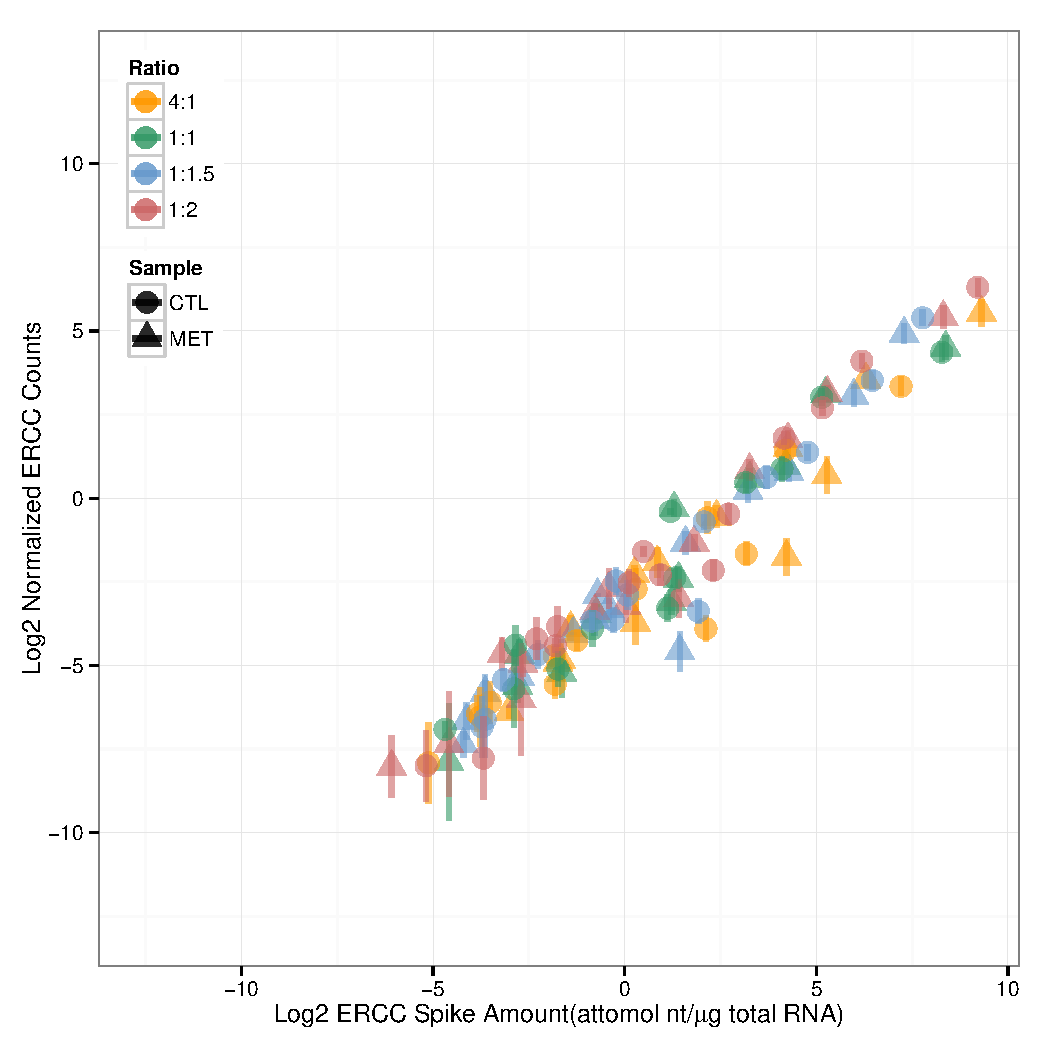
\includegraphics{erccdashboardVignette-ratPlotA}
\end{center}
For this particular experiment the relationship between abundance and signal for
the ERCC controls show that the measurement results span a 2$^{15}$ dynamic range.
These ERCC mixtures were designed to span a 2$^{20}$ dynamic range, but there was 
insufficient evidence to reliably quantify ERCC transcripts at low 
abundances.
\clearpage
\begin{center}
\begin{Schunk}
\begin{Sinput}
> exDat$Figures$rocPlot
\end{Sinput}
\end{Schunk}
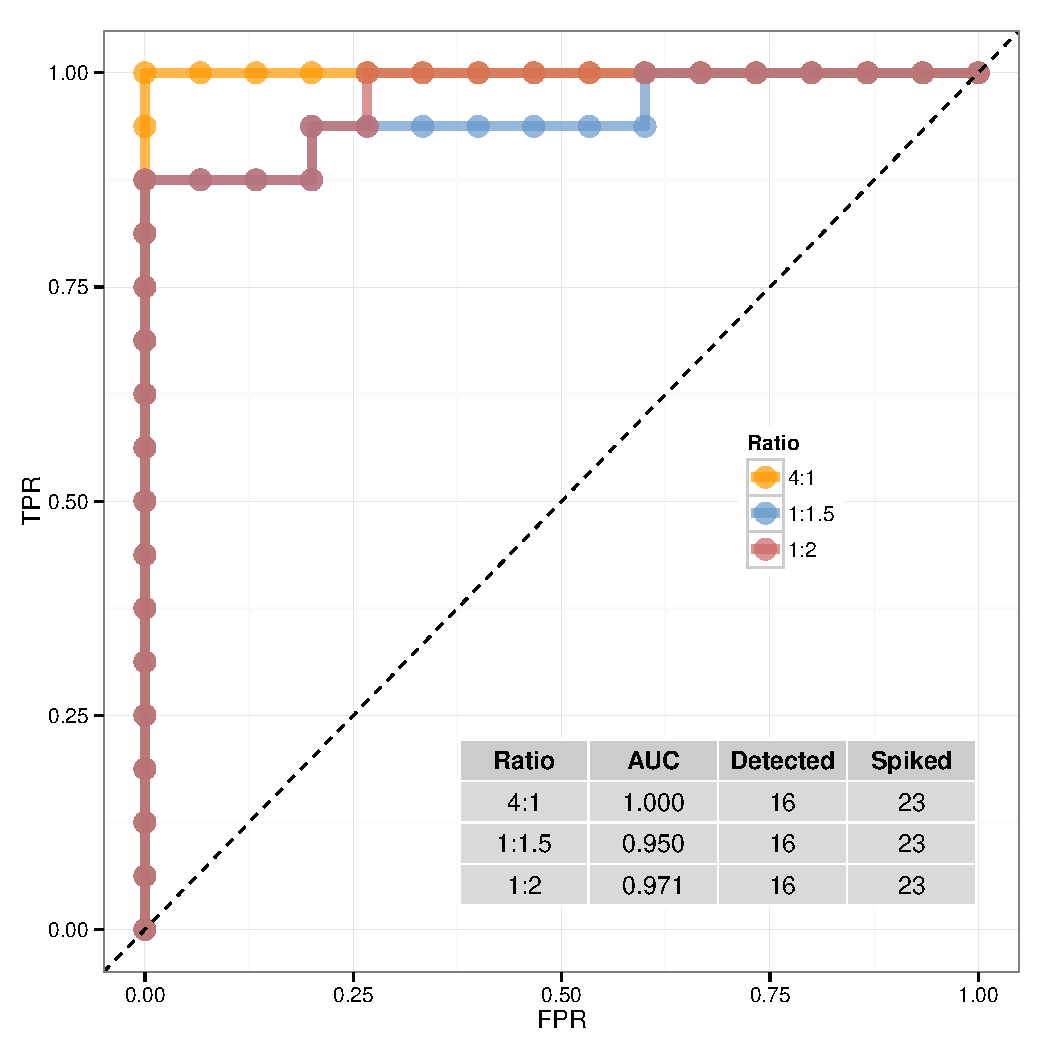
\includegraphics{erccdashboardVignette-ratPlotB}
\end{center}
The receiver operator characteristic (ROC) curve and the Area Under the Curve (AUC)
statistic provide evidence of the diagnostic power for detecting differential expression
in this rat toxicogenomics experiment. As expected with increased fold change,
diagnostic power increases. The AUC summary statistic for different experiments
can be used to compare diagnostic performance.
\clearpage
\begin{center}
\begin{Schunk}
\begin{Sinput}
> exDat$Figures$lodrERCCPlot
\end{Sinput}
\end{Schunk}
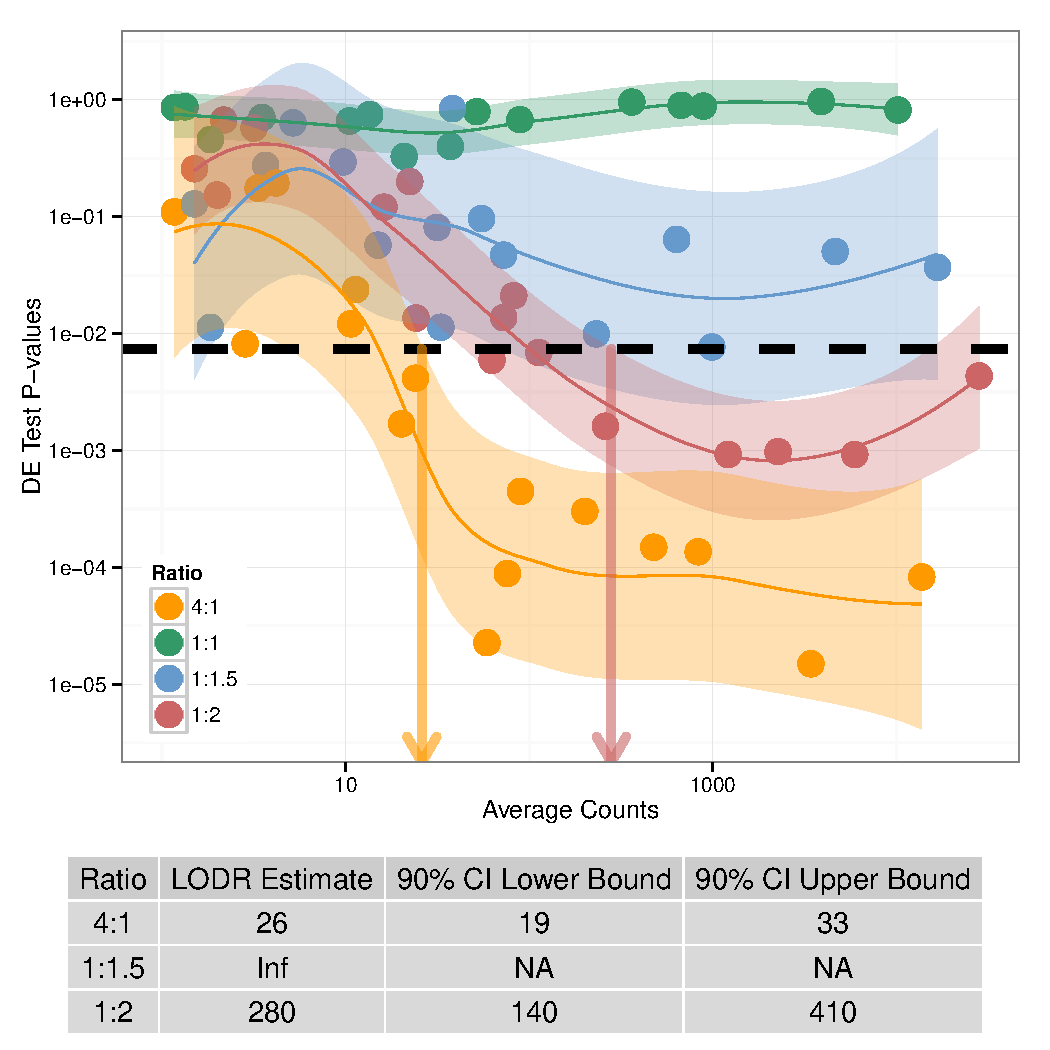
\includegraphics{erccdashboardVignette-ratPlotC}
\end{center}
By modeling the relationship between average signal and p-values we can obtain 
Limit of Detection of Ratios (LODR) estimates for each differential fold change 
(or Ratio,indicated by color) and a threshold p-value, p.thresh, indicated by 
the dotted black line. LODR values can be compared between
experiments to evaluate the ability to detect differences between samples as a function
of transcript abundance.
\clearpage
\begin{center}
\begin{Schunk}
\begin{Sinput}
> exDat$Figures$maPlot
\end{Sinput}
\end{Schunk}
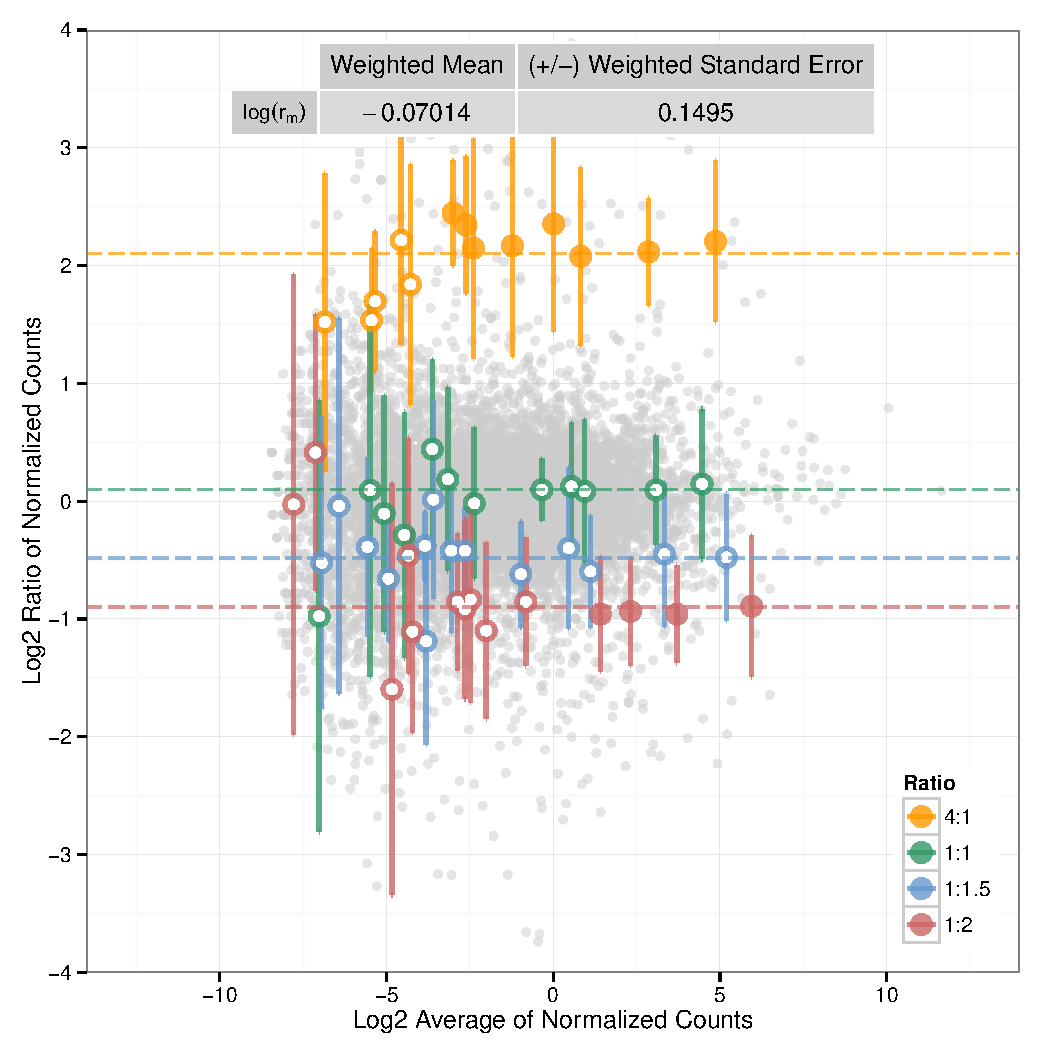
\includegraphics{erccdashboardVignette-ratPlotD}
\end{center}
An MA plot (Ratio of Signals vs Average Signals) shows the ratio measurements of
transcripts in the pair of samples as a function of abundance. The ERCC control 
ratios measurements are coded to indicate which controls are above a given LODR 
(solid circles) or below the LODR (open circles). This plot also shows the v
ariability in ratio measurements as a function of dynamic range and the bias in 
control ratio measurements (r$_m$), which is influenced by the mRNA fraction difference
between the pair of samples.

\section{SEQC Reference RNA (UHRR and HBRR) Examples}
All UHRR and HBRR experiments for the SEQC interlaboratory and interplatform 
analysis were performed with aliquots from single large samples of UHRR and 
HBRR. The count data and microarray data provided here are from experiments 
using the same original UHRR and HBRR samples.

\subsection{RNA-Seq UHRR vs. HBRR experiment analysis}
\begin{Schunk}
\begin{Sinput}
> exDat <- runDashboard(datType="count", isNorm = FALSE,
                        exTable=Lab5.ILM.UHRR.HBRR.countTable,
                        filenameRoot="Lab5", sample1Name = "UHRR", 
                        sample2Name = "HBRR", erccmix = "RatioPair",
                        erccdilution = 1, spikeVol = 50, 
                        totalRNAmass = 2.5*10^(3), choseFDR = 0.01)
\end{Sinput}
\begin{Soutput}
Initializing the exDat list structure...
choseFDR = 0.01 
repNormFactor is NULL 
Filename root is: Lab5.UHRR.HBRR 

Transcripts were removed with a mean count < 1 or more than 2 
replicates with 0 counts.
Original data contained  43919 transcripts. 
After filtering  39844 transcripts remain for  analysis.
A total of 2 out of 92 
ERCC controls were filtered from the data set
The excluded ERCCs are:
ERCC-00057 ERCC-00083

repNormFactor is NULL,
 Using Default Upper Quartile Normalization Method  - 75th percentile

normVec:
4048 7635 5739.25 12885 7033 6176 7059 7141.25
Check for sample mRNA fraction differences(r_m)...

Number of ERCC Controls Used in r_m estimate
90 

Outlier ERCCs for GLM r_m Estimate:
ERCC-00012 ERCC-00137 ERCC-00085 ERCC-00054 ERCC-00019

GLM log(r_m) estimate:
0.2836417 

GLM log(r_m) estimate weighted s.e.:
0.03764492 

Number of ERCCs in Mix 1 dyn range:  90 

Number of ERCCs in Mix 2 dyn range:  90 
These ERCCs were not included in the signal-abundance plot,
because not enough non-zero replicate measurements of these 
controls were obtained for both samples:

ERCC-00016 ERCC-00017 ERCC-00048 ERCC-00061 ERCC-00075
ERCC-00104 ERCC-00117 ERCC-00142 ERCC-00156 ERCC-00097
ERCC-00123 ERCC-00138


Saving dynRangePlot to exDat

Starting differential expression tests

Show log.offset
8.305978 8.940498 8.655084 9.463819 8.858369 8.728426 8.862059 8.873643 
Disp = 0.00099 , BCV = 0.0314 
Disp = 0.00104 , BCV = 0.0322 
[1] "Analyzing Gene # 2"
[1] "Analyzing Gene # 10"
[1] "Analyzing Gene # 100"
[1] "Analyzing Gene # 500"
[1] "Analyzing Gene # 1000"
[1] "Analyzing Gene # 2500"
[1] "Analyzing Gene # 5000"
[1] "Analyzing Gene # 10000"
[1] "Analyzing Gene # 15000"
[1] "Analyzing Gene # 20000"
[1] "Analyzing Gene # 25000"
[1] "Analyzing Gene # 30000"
[1] "Analyzing Gene # 35000"
[1] "Analyzing Gene # 40000"
[1] "Analyzing Gene # 2"
[1] "Analyzing Gene # 10"
[1] "Analyzing Gene # 100"
[1] "Analyzing Gene # 500"
[1] "Analyzing Gene # 1000"
[1] "Analyzing Gene # 2500"
[1] "Analyzing Gene # 5000"
[1] "Analyzing Gene # 10000"
[1] "Analyzing Gene # 15000"
[1] "Analyzing Gene # 20000"
[1] "Analyzing Gene # 25000"
[1] "Analyzing Gene # 30000"
[1] "Analyzing Gene # 35000"
[1] "Analyzing Gene # 40000"
Note: 'test.mat' not provided. Comparing each model 
from 'design.list' to first model in 'design.list', which must be the full model
[1] "Spline scaling factor: 1.09854245480117"
[1] "Spline scaling factor: 1.09834239703167"
[1] "Analyzing Gene # 2"
[1] "Analyzing Gene # 10"
[1] "Analyzing Gene # 2"
[1] "Analyzing Gene # 10"
Note: 'test.mat' not provided. Comparing each model 
from 'design.list' to first model in 'design.list', which must be the full model
[1] "Spline scaling factor: 1.09834239703167"
[1] "Finished DE testing"
[1] "Spline scaling factor: 1.09834239703167"

Finished examining dispersions

Threshold P-value
0.152249 
Threshold P-value is high for the chosen FDR of  0.01
The sample comparison indicates a large amount of 
 differential expression in the measured transcript 
 populations

Generating ROC curve and AUC statistics...

Area Under the Curve (AUC) Results:
  Ratio   AUC Detected Spiked
1   4:1 0.966       22     23
2 1:1.5 0.830       22     23
3   1:2 0.888       23     23

Estimating ERCC LODR
.............................................
  Ratio LODR Estimate 90% CI Lower Bound 90% CI Upper Bound
1   4:1            20                6.9                 26
3 1:1.5           160                 70                190
4   1:2            38                 23                 42

 ERCC LODR estimates are available
   Fold Ratio Abund Log2Abund
1 4.000   4:1    20 -8.494768
2 1.000   1:1    NA        NA
3 0.667 1:1.5   160 -5.494768
4 0.500   1:2    38 -7.568769

LODR estimates are available to code ratio-abundance plot

Saving main dashboard plots to pdf file...
Saving exDat list to .RData file...
Analysis completed.
\end{Soutput}
\end{Schunk}
\clearpage
\begin{center}
\begin{Schunk}
\begin{Sinput}
> exDat$Figures$dynRangePlot
\end{Sinput}
\end{Schunk}
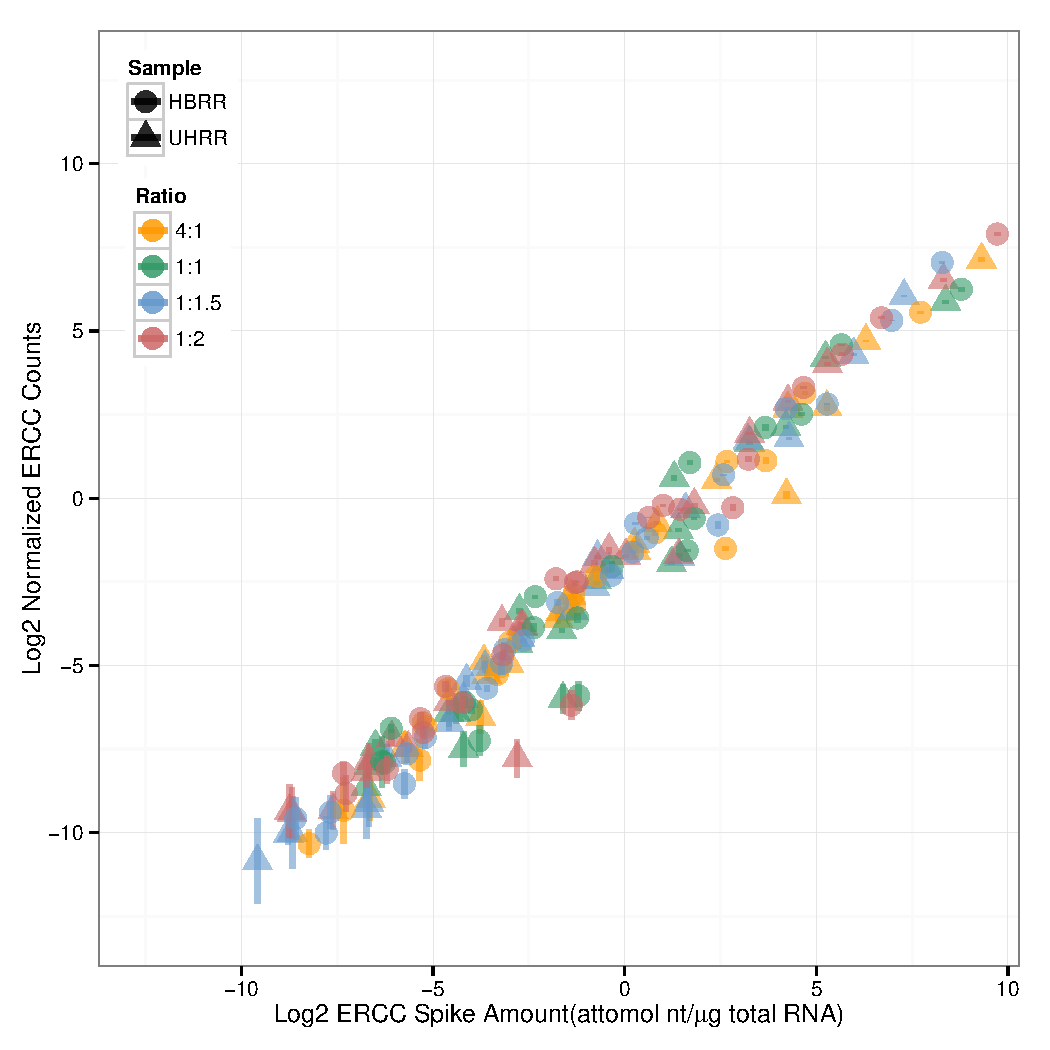
\includegraphics{erccdashboardVignette-seqcCountPlotA}
\end{center}
Compared with the rat toxicogenomics experiment the UHRR/HBRR experiment from Lab 5 
captures the full dynamic range of 2$^{20}$ in the ERCC mixture design. This 
difference can be attributed to an much greater sequencing depth in the 
UHRR/HBRR experiments at each laboratory (full fluidic capacity of an 
instrument) compared to the MET-CTL rat toxicogenomics experiment. This 
difference is apparent in the total reads vectors for the two different 
experiments:
\begin{Schunk}
\begin{Sinput}
> COH.RatTox.ILM.MET.CTL.totalReads
\end{Sinput}
\begin{Soutput}
[1] 41423502 46016148 44320280 38400362 47511484 33910098
\end{Soutput}
\begin{Sinput}
> Lab5.ILM.UHRR.HBRR.totalReads
\end{Sinput}
\begin{Soutput}
[1] 138786892 256006510 199468322 431933806 247985592
[6] 219383270 251265814 257508210
\end{Soutput}
\end{Schunk}
\clearpage
\begin{center}
\begin{Schunk}
\begin{Sinput}
> exDat$Figures$rocPlot
\end{Sinput}
\end{Schunk}
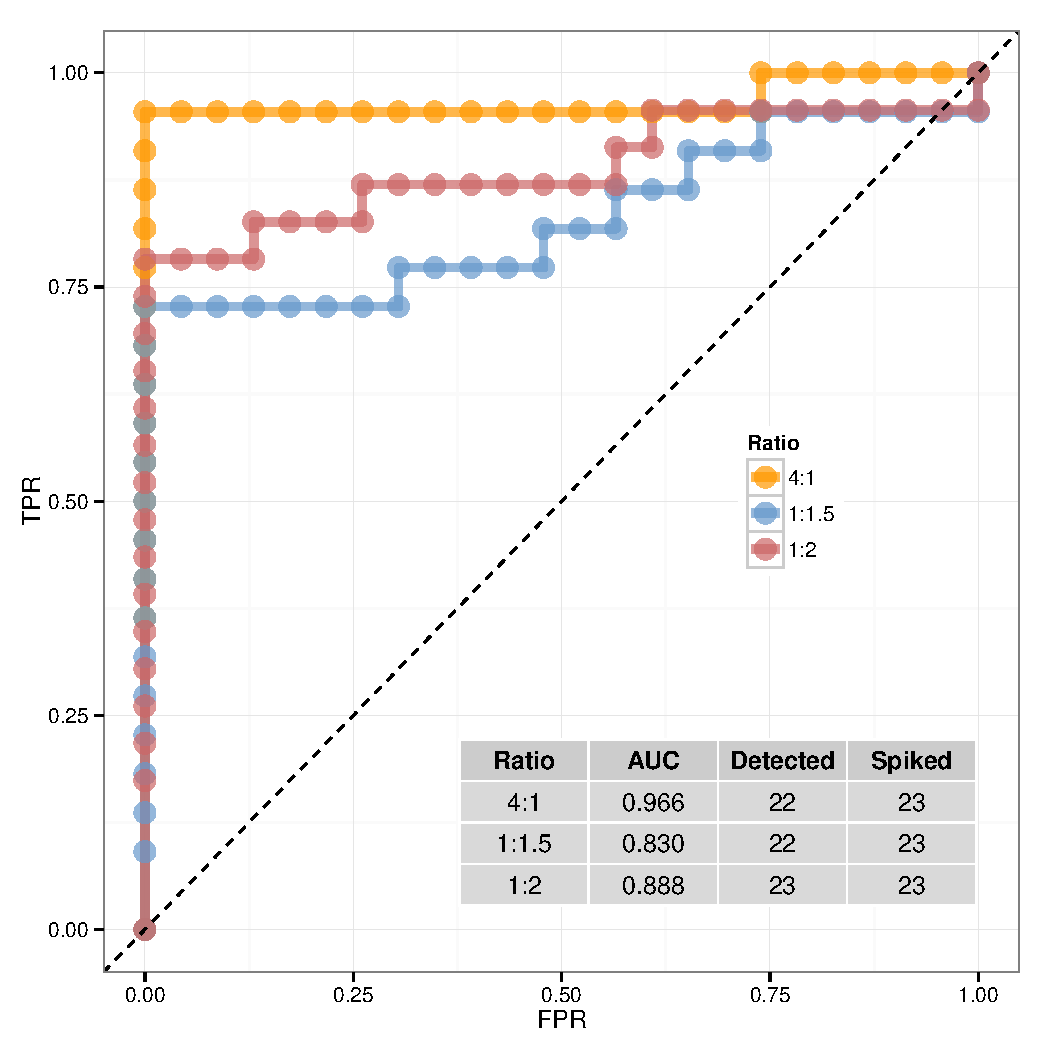
\includegraphics{erccdashboardVignette-seqcCountPlotB}
\end{center}

Given the sequencing depth of the Lab 5 UHRR/HBRR experiment it is unsurprising that 
the ROC curve results show that almost all of the spiked ERCC transcripts were 
detected and tested for differential expression. At first glance, one may attempt
to compare these ROC curve and AUC results to the rat toxicogenomics results, but
this is ill-advised because the samples under comparison are different. Not only
is the sequencing depth different for the two experiments, but the UHRR/HBRR 
sample transcripts also have high levels of differential expression, whereas 
the rat MET/CTL samples have much lower levels of differential expression. This
difference in differential expression is shown in the spread and density of the 
points representing the endogenous transcripts in the MA plots for each experiment.
 
\clearpage
\begin{center}
\begin{Schunk}
\begin{Sinput}
> exDat$Figures$lodrERCCPlot
\end{Sinput}
\end{Schunk}
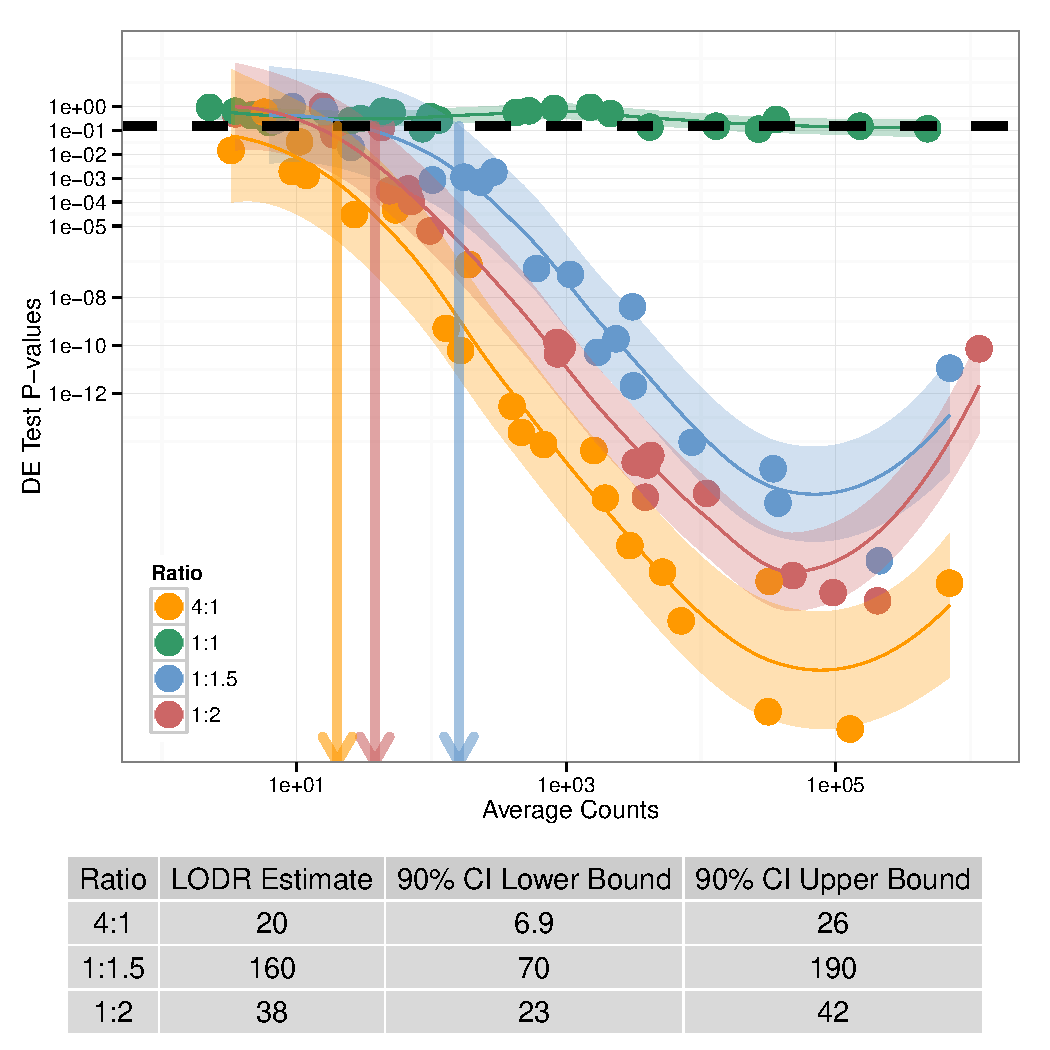
\includegraphics{erccdashboardVignette-seqcCountPlotC}
\end{center}

Much lower LODR estimates are found in the Lab 5 UHRR/HBRR experiment compared to the 
rat experiment. One can also see that the p-values in this analysis are much smaller
than those in the rat experiment due to the large amount of differentially expressed
transcripts in the UHRR/HBRR comparison.
\clearpage
\begin{center}
\begin{Schunk}
\begin{Sinput}
> exDat$Figures$maPlot
\end{Sinput}
\end{Schunk}
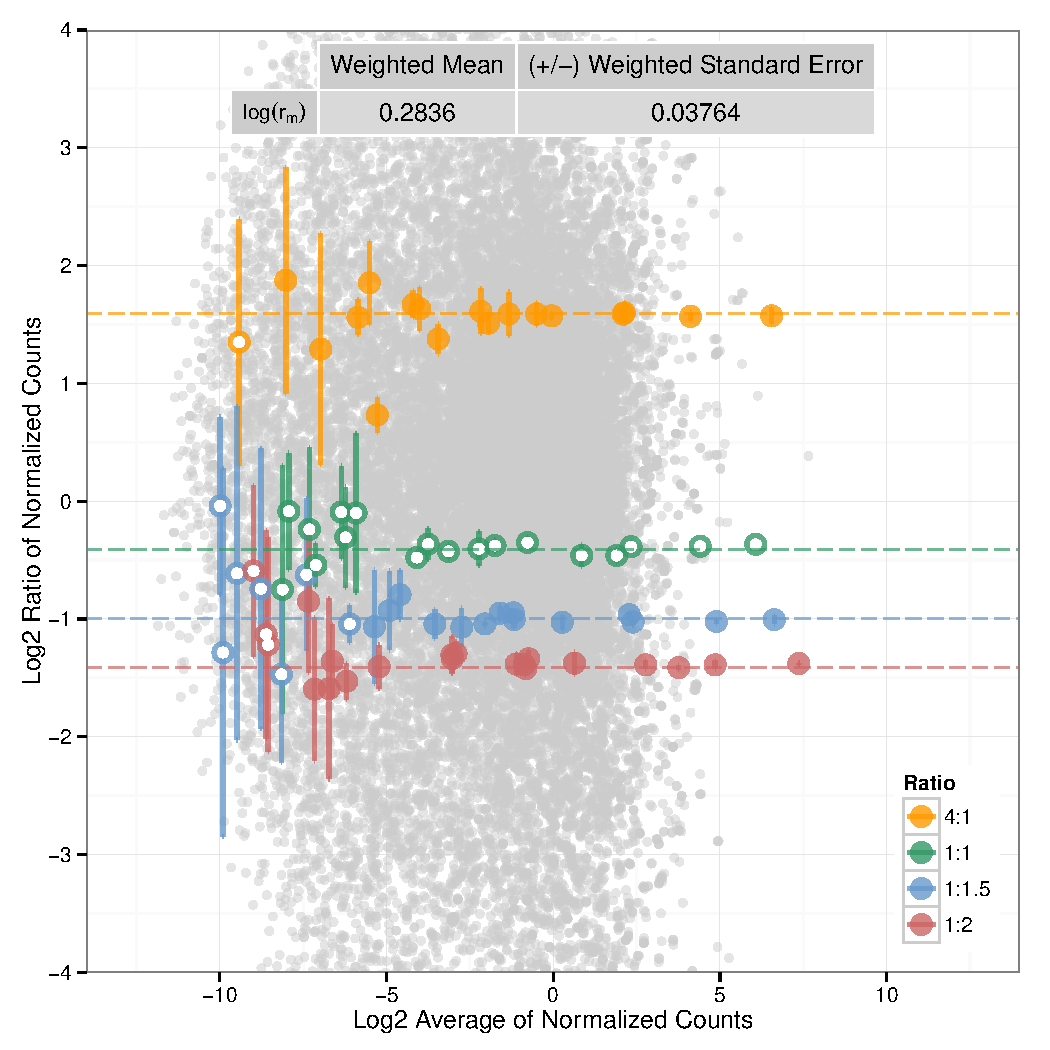
\includegraphics{erccdashboardVignette-seqcCountPlotD}
\end{center}

Variability in the ratio measurements in this experiment is much lower than in
the rat experiment. This is due to the nature of the replication in the two experiments.
In the rat experiment the 3 replicates for each condition represent biological 
replicates, while in the UHRR/HBRR experiment the 4 replicates represent library 
preparation replicates of the same source samples and each library replicate count column was 
a sum of multiple fluidic replicates of the same library replicate.
The bias in control ratios in this experiment is much greater than what was observed in
the rat experiment. This bias is likely due to the known mRNA fraction difference
between the UHRR and HBRR RNA samples.

\clearpage
\subsection{Microarray UHRR vs. HBRR experiment analysis}
Unnormalized fluorescent signals are expected for erccdashboard analysis of 
microarray data, the data will be log2 transformed for DE testing with the limma
package. The repNormFactor variable should
be NULL for microarray analysis, and repNormFactor is set to NULL if it is 
missing in the list of arguments for the runDashboard function. Each array 
replicate is normalized by the 75th quantile fluoresence intensity 
value of that array.
\begin{Schunk}
\begin{Sinput}
> exDat <- runDashboard(datType="array", isNorm = F,
                        exTable=Lab10.array.UHRR.HBRR,
                        filenameRoot = "Lab10.array",
                        sample1Name = "UHRR", sample2Name="HBRR",
                        erccmix = "RatioPair", erccdilution = 1, 
                        spikeVol = 50, totalRNAmass = 2.5*10^(3), choseFDR=0.01)
\end{Sinput}
\begin{Soutput}
Initializing the exDat list structure...
choseFDR = 0.01 
repNormFactor is NULL 
Filename root is: Lab10.array.UHRR.HBRR 

Using 75th percentile (upper quartile) intensity to normalize each array

normVec:
694.35 758.9 705 570.55 640.25 641.3
Check for sample mRNA fraction differences(r_m)...

datType is array, using 1:1 ERCC controls for r_m estimate

Number of ERCC Controls Used in r_m estimate
15 

Outlier ERCCs for GLM r_m Estimate:
ERCC-00035 ERCC-00042

GLM log(r_m) estimate:
0.2070304 

GLM log(r_m) estimate weighted s.e.:
0.09446045 

Number of ERCCs in Mix 1 dyn range:  59 

Number of ERCCs in Mix 2 dyn range:  59 

datType is array, no linear model fit for ERCC specific effects

rangeResidPlot is empty

Saving dynRangePlot to exDat

Finished DE testing

Generating ROC curve and AUC statistics...

Area Under the Curve (AUC) Results:
  Ratio   AUC Detected Spiked
1   4:1 0.933       14     23
2 1:1.5 0.929       14     23
3   1:2 0.917       16     23

Estimating ERCC LODR
.............................................
  Ratio LODR Estimate 90% CI Lower Bound 90% CI Upper Bound
1   4:1          <150               <150               <150
3 1:1.5           200               <160                210
4   1:2           150               <130                160

 ERCC LODR estimates are available
   Fold Ratio Abund Log2Abund
1 4.000   4:1   150 -2.155731
2 1.000   1:1    NA        NA
3 0.667 1:1.5   200 -1.740694
4 0.500   1:2   150 -2.155731

LODR estimates are available to code ratio-abundance plot

Saving main dashboard plots to pdf file...
Saving exDat list to .RData file...
Analysis completed.
\end{Soutput}
\end{Schunk}
\clearpage
\begin{center}
\begin{Schunk}
\begin{Sinput}
> exDat$Figures$dynRangePlot
\end{Sinput}
\end{Schunk}
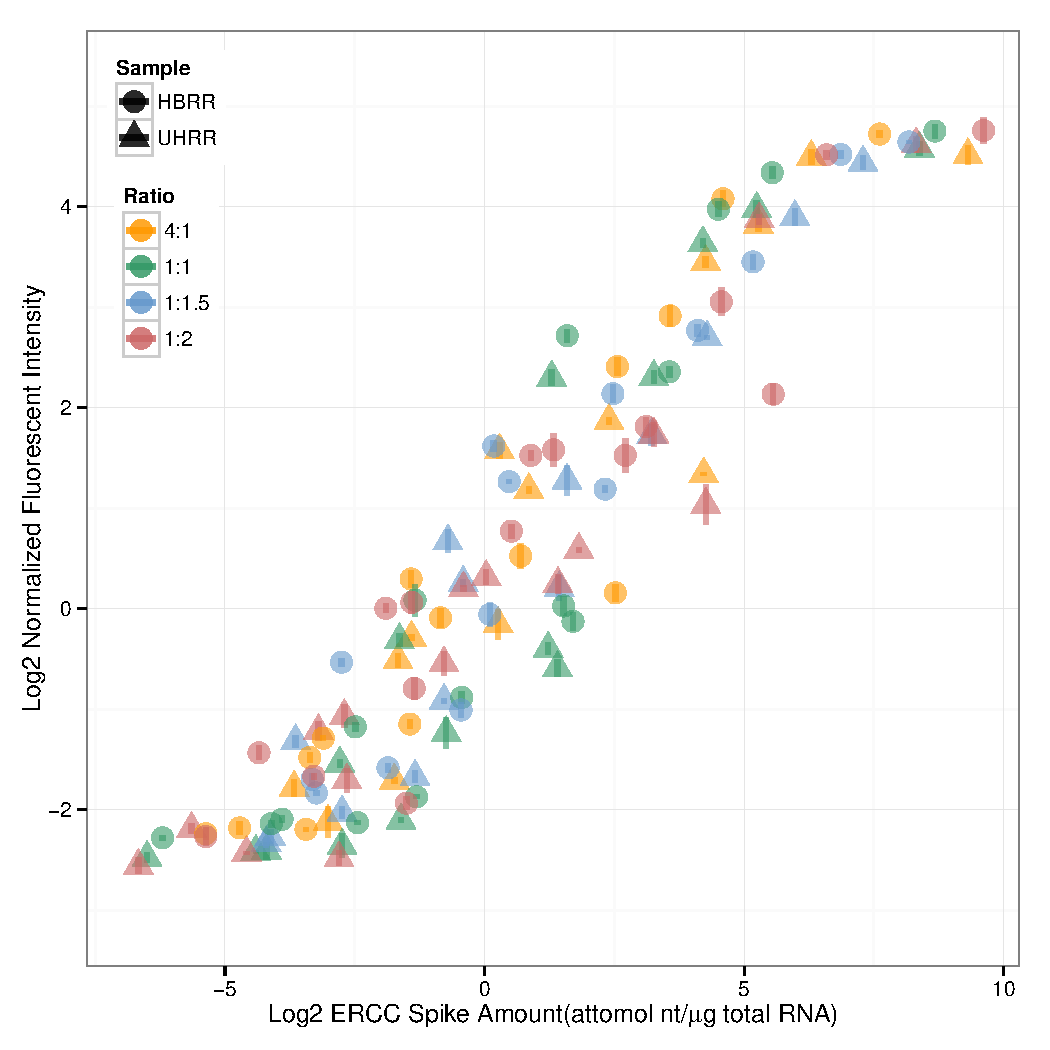
\includegraphics{erccdashboardVignette-seqcArrayPlotA}
\end{center}

The dynamic range of the microarray experiment on reference RNA samples was 2$^{10}$.
This figure shows the signal compression for high abundance transcripts.
\clearpage
\begin{center}
\begin{Schunk}
\begin{Sinput}
> exDat$Figures$rocPlot
\end{Sinput}
\end{Schunk}
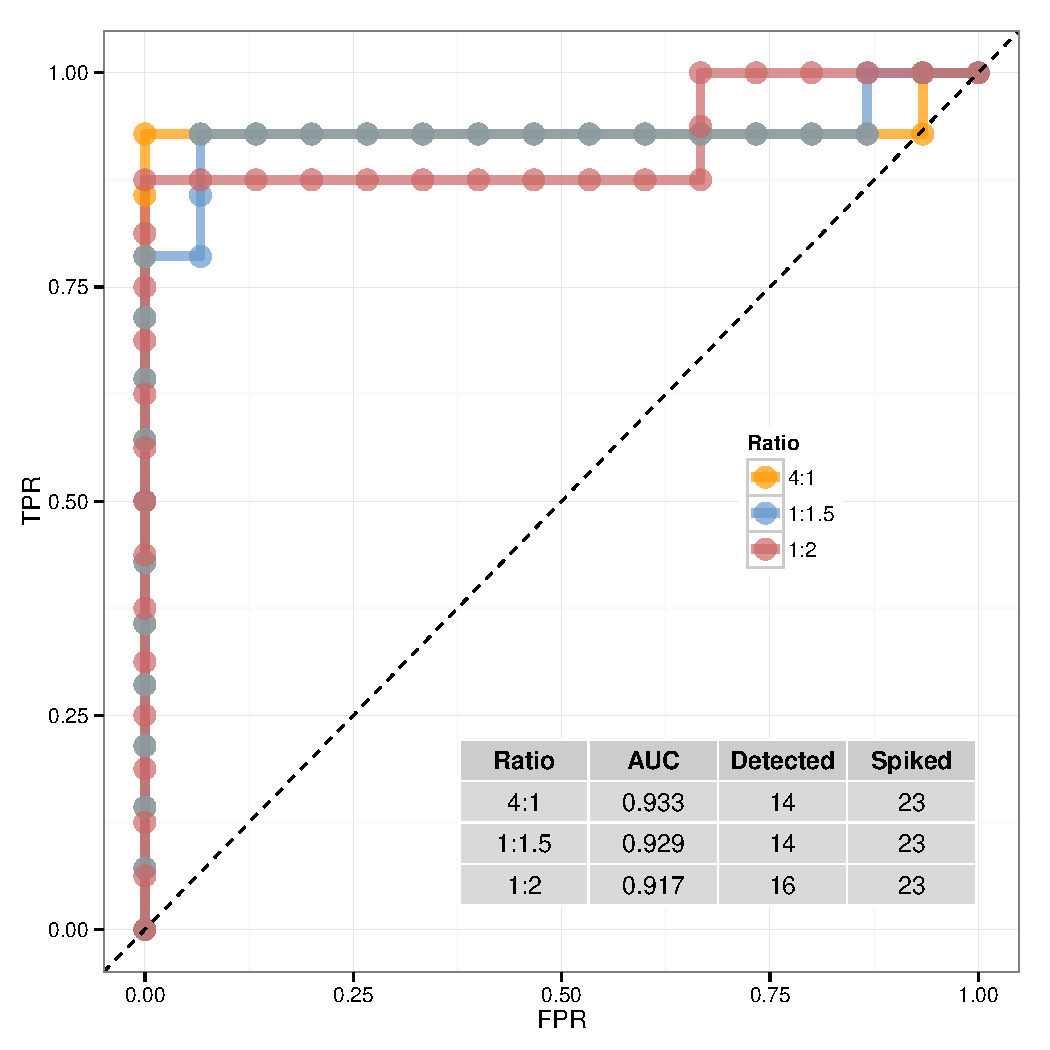
\includegraphics{erccdashboardVignette-seqcArrayPlotB}
\end{center}

Comparison of these microarray ROC curves and AUC statistics to the results in the RNA-Seq 
UHRR/HBRR experiment from Lab 5 show similar diagnostic power 
for the two platforms. Fewer controls were detected above background in the microarray experiment, and this should be considered when comparing the diagnostic performance
of the two platforms. More stringent filtering of RNA-Seq data would likely lead to improved diagnostic
performance.
\clearpage
\begin{center}
\begin{Schunk}
\begin{Sinput}
> exDat$Figures$lodrERCCPlot
\end{Sinput}
\end{Schunk}
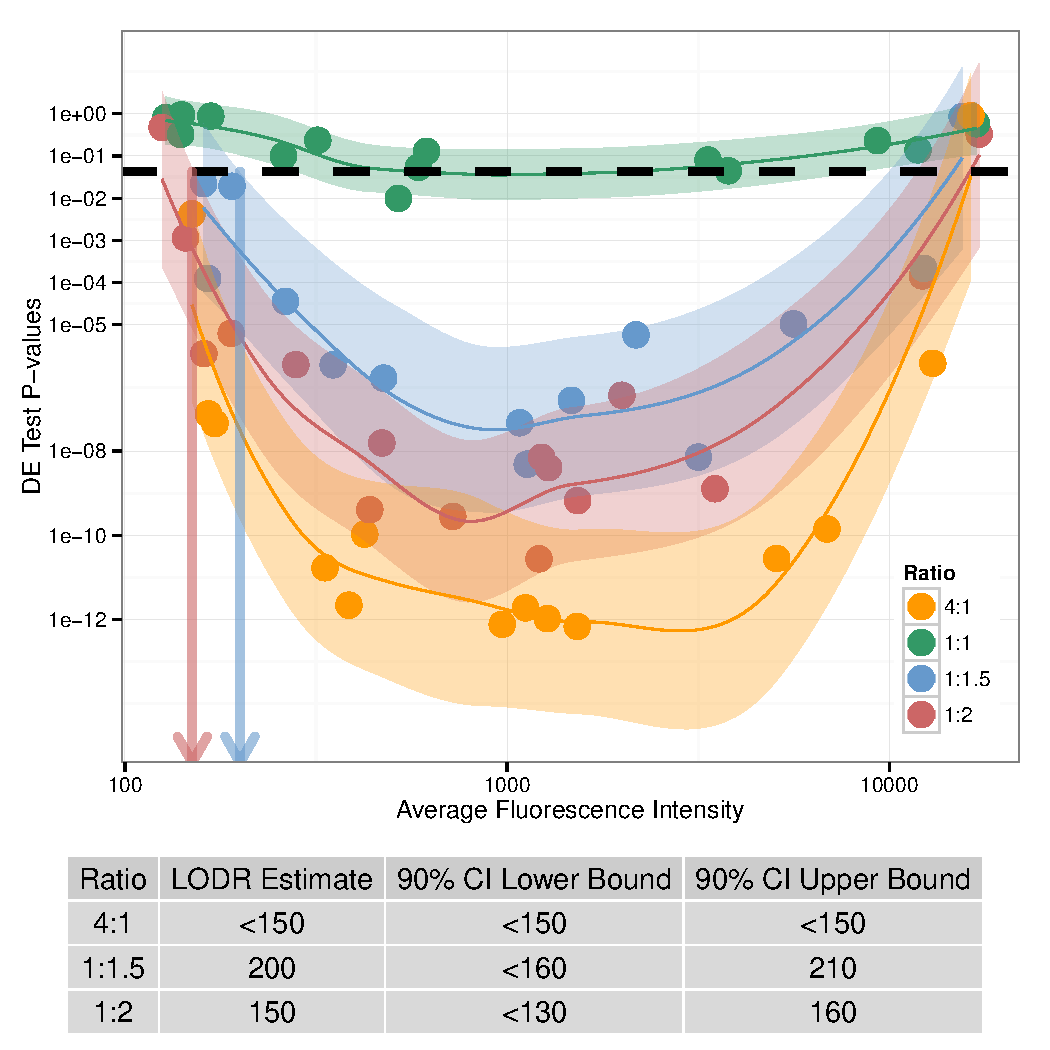
\includegraphics{erccdashboardVignette-seqcArrayPlotC}
\end{center}

LODR estimates for microarray data are derived from the intersection with the 
threshold p-value at the lowest signal. The same FDR was chosed for the RNA-Seq 
and microarray measurements of the UHRR/HBRR samples, it is interesting to note 
that different threshold p-values were derived for each type of experiment using
the same FDR = 0.01, p.thresh = 0.1518 for RNA-Seq at Lab 5 and 
p.thresh = 0.0430 for the microarray experiment.
\clearpage
\begin{center}
\begin{Schunk}
\begin{Sinput}
> exDat$Figures$maPlot
\end{Sinput}
\end{Schunk}
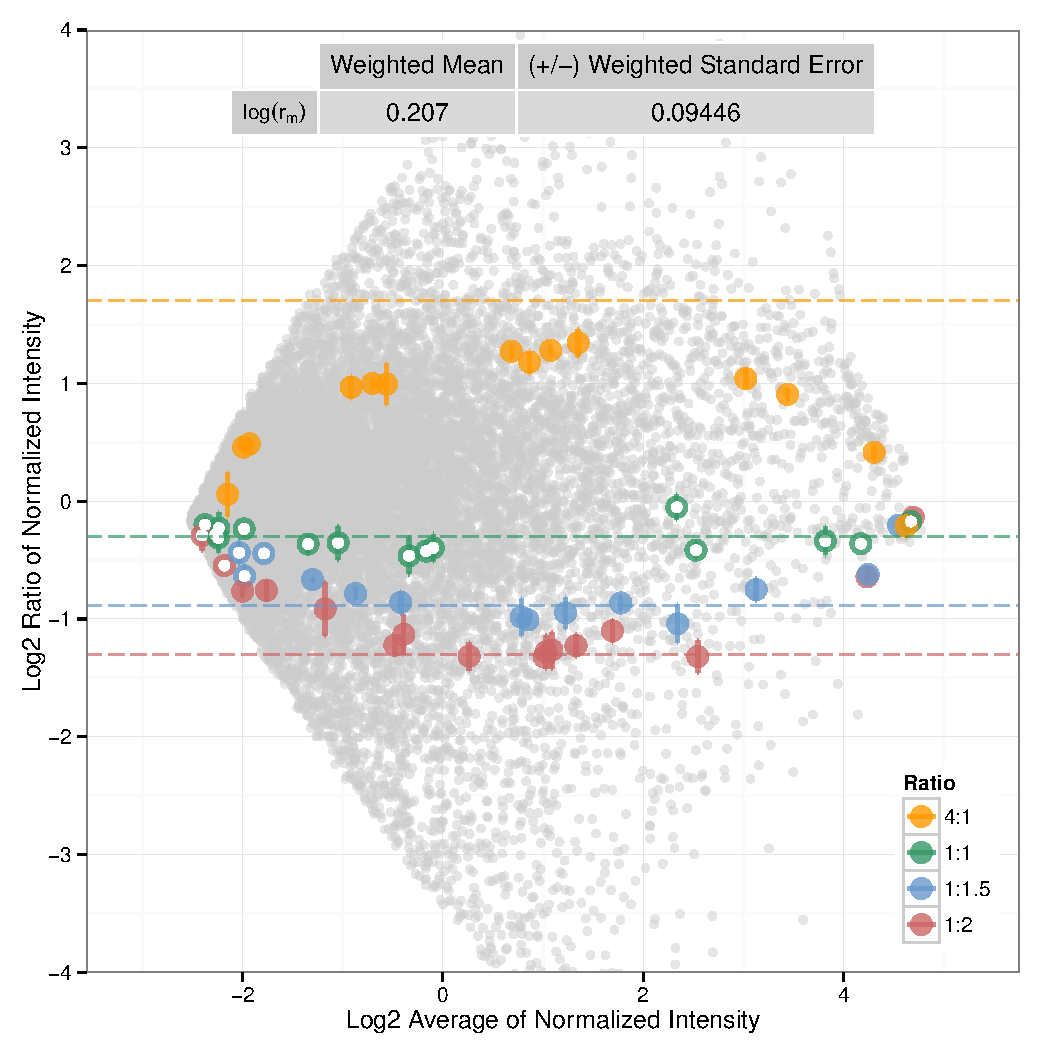
\includegraphics{erccdashboardVignette-seqcArrayPlotD}
\end{center}

The variability and bias in the control ratio measurements 
in the microarray data measurement of UHRR/HBRR are similar to the observations in
the RNA-Seq UHRR/HBRR experiment.

\section{Comparison of Performance Between Experiments}
The performance metrics provided here derived from measurements of ERCC ratios in
gene expression experiments (AUC, LODR, r$_m$, and the standard deviations of 
the ERCC ratio measurements) can be used to assess performance between experiments within
the same laboratory, or between different laboratories or technology platforms.

\section{Analysis Details: Advanced Use of Functions in runDashboard}
The analysis functions contained in the convenience wrapper function 
\verb|runDashboard| can also be used directly by the user.
Comments are provided above each analysis step included in \verb|runDashboard| to
describe the purpose and ordering constraints.
View the runDashboard script to see comments describing the analysis functions and the ordering constraints:
\begin{Schunk}
\begin{Sinput}
> runDashboard
\end{Sinput}
\begin{Soutput}
function (datType = NULL, isNorm = F, exTable = NULL, repNormFactor = NULL, 
    filenameRoot = NULL, sample1Name = NULL, sample2Name = NULL, 
    erccmix = "RatioPair", erccdilution = 1, spikeVol = 1, totalRNAmass = 1, 
    choseFDR = 0.05, ratioLim = c(-4, 4), signalLim = c(-14, 
        14), userMixFile = NULL) 
{
    exDat <- initDat(datType = datType, isNorm = isNorm, exTable = exTable, 
        repNormFactor = repNormFactor, filenameRoot = filenameRoot, 
        sample1Name = sample1Name, sample2Name = sample2Name, 
        erccmix = erccmix, erccdilution = erccdilution, spikeVol = spikeVol, 
        totalRNAmass = totalRNAmass, choseFDR = choseFDR, ratioLim = ratioLim, 
        signalLim = signalLim, userMixFile = userMixFile)
    exDat <- est_r_m(exDat)
    exDat <- dynRangePlot(exDat)
    if (erccmix == "RatioPair") {
        exDat <- withinMixRatios(exDat)
    }
    exDat <- geneExprTest(exDat)
    exDat <- erccROC(exDat)
    exDat = estLODR(exDat, kind = "ERCC", prob = 0.9)
    exDat <- annotLODR(exDat)
    saveERCCPlots(exDat)
    cat("\nSaving exDat list to .RData file...")
    nam <- paste(exDat$sampleInfo$filenameRoot, "exDat", sep = ".")
    assign(nam, exDat)
    to.save <- ls()
    save(list = to.save[grepl(pattern = nam, x = to.save)], file = paste0(exDat$sampleInfo$filenameRoot, 
        ".RData"))
    cat("\nAnalysis completed.")
    return(exDat)
}
<environment: namespace:erccdashboard>
\end{Soutput}
\end{Schunk}

\subsection{Flexibility in Differential Expression Testing}
The \verb|geneExprTest| function wraps the QuasiSeq differential expression 
testing package for datType = "count" or uses the limma package for differential
expression testing if datType = "array". The function uses the DE testing 
p-value results and choseFDR parameter to select a threshold p-value for LODR 
estimation.
In the case of count data if a correctly formatted csv file is provided with the
necessary DE test results, then geneExprTest will bypass DE testing (with 
reduced runtime). The function will look for a csv file with the name 
"filenameRoot.quasiSeq.res.csv" and columns with names "Feature", "pvals", and 
"qvals" must be in the file.

\subsection{Options for LODR Estimation}
The default behavior of runDashboard is to use the \verb|estLODR| function to
obtain an LODR estimate using empirical data from the ERCCs and a model-based 
simulation using the endogenous genes in the sample. The type of LODR estimation
is selected using the argument kind in the \verb|estLODR| function. The other 
parameter that may be adjusted is the probability for the LODR estimate, in the 
default analysis prob = 0.9 is selected.

\subsection{Options for Printing Plots to File}
The function savePlots will save selected figures to a pdf file. The default 
is the 4 manuscript figures to a single page (plotsPerPg = "manuscript"). 
If plotsPerPg = "single" then each plot is placed on an 
individual page in one pdf file. If plotlist is not defined (plotlist = NULL)
then all plots in \verb|exDat$Figures| are printed to the file.

To print 4 plots from manuscript to a single page pdf file use 
plotsPerPg = "manuscript" in the \verb|saveERCCPlots| function or to create a 
multiplepage pdf of all plots produced use plotsPerPg = "single". 

\subsection{Analysis of Alternative Spike-in Designs}
By default the package is configured to analyze the ERCC ratio mixtures produced
by Ambion (ERCC ExFold RNA Spike-In Mixes, Catalog Number 4456739). This pair of
control ratio mixtures were designed to have 1:1, 4:1, 1:1.5, and 1:2 ratios of 92
distinct RNA transcripts (23 different RNA control sequences are in each of these 
four ratio subpools). Alternative ERCC RNA control ratio mixture designs can be 
produced using the NIST DNA Plasmid Library for External Spike-in Controls (NIST 
Standard Reference Material 2374, 
https://www-s.nist.gov/srmors/certificates/2374.pdf). For example, a pair of RNA
control mixtures could be created with a ternary ratio design, three subpools of 
RNA controls with either no change (1:1) or 2-fold increased (2:1) and 2-fold
decreased (1:2) relative abundances between the pair of mixtures (Mix 1/Mix 2).
To use alternative spike-in mixture designs with the dashboard a csv file must
be provided to the package with the argument userMixFile for the initDat function. 

If all samples from both conditions were only spiked with a single ERCC mixture 
(e.g. Ambion Catalog Number 4456740, ERCC RNA Spike-In Mix) a limited subset of 
the package functions can be used (\verb|initDat|, \verb|est_r_m|, and 
\verb|dynRangePlot|. For \verb|initDat| use ERCCMixes="Single" and \verb|est_r_m| and 
\verb|dynRangePlot| functions can then be used to examine the mRNA fraction 
differences for the pair of samples and evaluate the dynamic range of the 
experiment. 

\section{Notes on R version and session information}
The results shown in this R vignette are the same as the results shown in our
manuscript and were obtained in R version 3.0.2 with the following session 
information.
\begin{Schunk}
\begin{Sinput}
> sessionInfo()
\end{Sinput}
\begin{Soutput}
R version 3.1.0 (2014-04-10)
Platform: x86_64-apple-darwin10.8.0 (64-bit)

locale:
[1] en_US.UTF-8/en_US.UTF-8/en_US.UTF-8/C/en_US.UTF-8/en_US.UTF-8

attached base packages:
[1] splines   grid      stats     graphics  grDevices
[6] utils     datasets  methods   base     

other attached packages:
[1] erccdashboard_0.9.8 gridExtra_0.9.1    
[3] ggplot2_0.9.3.1    

loaded via a namespace (and not attached):
 [1] bitops_1.0-6       caTools_1.17      
 [3] colorspace_1.2-4   digest_0.6.4      
 [5] edgeR_3.6.1        gdata_2.13.3      
 [7] gplots_2.13.0      gtable_0.1.2      
 [9] gtools_3.4.0       KernSmooth_2.23-12
[11] labeling_0.2       lattice_0.20-29   
[13] limma_3.20.1       locfit_1.5-9.1    
[15] MASS_7.3-32        Matrix_1.1-3      
[17] mgcv_1.7-29        munsell_0.4.2     
[19] nlme_3.1-117       plyr_1.8.1        
[21] proto_0.3-10       QuasiSeq_1.0-4    
[23] qvalue_1.38.0      Rcpp_0.11.1       
[25] reshape2_1.4       ROCR_1.0-5        
[27] scales_0.2.4       stringr_0.6.2     
[29] tcltk_3.1.0        tools_3.1.0       
\end{Soutput}
\end{Schunk}
 
\end{document}
